\documentclass[conference]{IEEEtran}
\IEEEoverridecommandlockouts
\usepackage{cite}
\usepackage{amsmath}
\usepackage{newtxtext,newtxmath}
\usepackage{graphicx}
\usepackage{booktabs}
\usepackage{multirow}
\usepackage{xcolor}
\usepackage{url}
\usepackage[hidelinks]{hyperref}
\hypersetup{
  pdftitle={Fault Diagnosis or Experiment Recognition? A Leakage-Aware Evaluation of Machine Learning for Grid-Connected PV Fault Diagnosis},
  pdfauthor={Haider Md. Faiyaz Hussain Shahi},
  pdfkeywords={photovoltaic systems, fault diagnosis, machine learning, data leakage, grid-connected inverter}
}

\begin{document}

\title{Fault Diagnosis or Experiment Recognition? A Leakage-Aware Evaluation of Machine Learning for Grid-Connected PV Fault Diagnosis}

\author{\IEEEauthorblockN{Haider Md. Faiyaz Hussain Shahi}
\IEEEauthorblockA{\textit{Independent Researcher} \\
shahihussainofficial1@gmail.com}
}

\maketitle

\begin{abstract}
Machine learning classifiers trained on the public GPVS-Faults dataset routinely report near-perfect accuracy in diagnosing faults of grid-connected photovoltaic (PV) systems. We show that this figure measures the ability to recognize \emph{which experiment} a measurement window comes from rather than \emph{which fault} is present. Under the commonly used protocol, in which every window of a recording is labeled with that recording's fault class and windows are split randomly, a random forest reaches 100\% accuracy. It reaches the same 100\% when it is trained and tested exclusively on data recorded \emph{before} any fault was injected, i.e., when there is no fault to diagnose. We then evaluate five classifiers under progressively stricter protocols: onset-aware labels, temporally blocked cross-validation with a purge gap, and cross-operating-mode transfer (MPPT$\leftrightarrow$IPPT). Under cross-mode transfer, macro-F1 falls to 0.17--0.32 for all models. Expressing each feature as a deviation from a short healthy reference period of the same installation (baseline referencing) raises the best cross-mode macro-F1 to 0.49. A training-free detector built on the same referenced features, calibrated on MPPT data only, attains a 0.7\% false-alarm rate in both modes and detects PV open-circuit, feedback-sensor and inverter faults in 67--99\% of post-fault windows, while partial shading and MPPT-controller faults remain undetected. We release the code and evaluation protocol to support reproducible benchmarking.
\end{abstract}

\begin{IEEEkeywords}
photovoltaic systems, fault diagnosis, machine learning, data leakage, explainable AI, grid-connected inverter
\end{IEEEkeywords}

\section{Introduction}
Undetected faults in photovoltaic (PV) systems reduce energy yield, accelerate component degradation and, in the case of arc and ground faults, create fire and safety hazards~\cite{mellit2018review,pillai2018review,madeti2017faults}. Data-driven fault detection and diagnosis (FDD) has therefore attracted considerable attention, with random forests~\cite{chen2018rf}, graph-based semi-supervised learning~\cite{zhao2015graph} and convolutional neural networks~\cite{aziz2020cnn} reporting high accuracies on simulated and experimental data.

Public experimental benchmarks are scarce. The GPVS-Faults dataset of Bakdi \emph{et al.}~\cite{bakdi2021realtime,bakdi2020gpvs} is one of the few that contains high-frequency measurements of a laboratory grid-connected PV system subjected to seven fault types under two operating modes, and it has become a reference for supervised and unsupervised methods~\cite{wali2021explainable,jorry2026kernel}. Supervised approaches on this dataset have reported accuracies of up to 100\%~\cite{wali2021explainable}.

Such figures are only meaningful if the evaluation protocol prevents the classifier from exploiting information that would be unavailable in deployment, a problem known as data leakage~\cite{kaufman2012leakage,kapoor2023leakage}. Two properties of GPVS-Faults make it particularly vulnerable. First, each fault type is represented by a single recording per operating mode, so ``fault class'' and ``recording'' are confounded. Second, the fault is injected only halfway through each recording; the first half is physically fault-free. A classifier can therefore score highly by learning the operating point, irradiance and temperature of each recording, a form of shortcut learning~\cite{geirhos2020shortcut}.

The contributions of this paper are:
\begin{enumerate}
\item A simple sanity check in which classifiers reach 100\% ``fault diagnosis'' accuracy on GPVS-Faults using only pre-fault data, showing that the standard protocol rewards experiment recognition.
\item A sequence of increasingly strict evaluation protocols (onset-aware labels, temporally blocked cross-validation with a purge gap, and cross-operating-mode transfer), on which we benchmark five classifiers and three feature sets.
\item \emph{Baseline referencing}, which expresses compact physics-informed features relative to a short healthy reference period of the same installation and roughly doubles cross-mode macro-F1.
\item A training-free, interpretable detector that transfers across operating modes with a 0.7\% false-alarm rate, together with per-fault detection rates and delays that identify which faults remain an open problem.
\end{enumerate}

\section{Related Work}
\subsection{PV Fault Detection and Diagnosis}
Reviews~\cite{mellit2018review,pillai2018review,madeti2017faults} classify PV FDD methods into model-based techniques, which compare measurements against an electrical model, and data-driven techniques, which learn decision boundaries from labeled or healthy data. Chen \emph{et al.}~\cite{chen2018rf} used array voltage and string currents with a random forest; Zhao \emph{et al.}~\cite{zhao2015graph} exploited unlabeled data through graph-based learning; Aziz \emph{et al.}~\cite{aziz2020cnn} classified array faults from scalograms with a CNN.

\subsection{Work on GPVS-Faults}
Bakdi \emph{et al.}~\cite{bakdi2021realtime} introduced the dataset together with an unsupervised PCA--kernel-density detector based on Kullback--Leibler divergence. Wali and Khan~\cite{wali2021explainable} extracted mean, standard deviation, minimum and maximum of all 13 signals over 200-sample batches, labeled every batch of a recording with the recording's fault class, split the batches randomly 70:30, and reported 100\% accuracy with a random forest explained by SHAP. Jorry \emph{et al.}~\cite{jorry2026kernel} proposed unsupervised kernel-norm monitoring calibrated on healthy data under IPPT mode. To our knowledge, no prior work on this dataset has quantified how much of the reported supervised accuracy is due to experiment identity.

\subsection{Leakage and Shortcut Learning}
Leakage occurs when training data contain information about the test target that will not be available at prediction time~\cite{kaufman2012leakage}; it has been identified as a cause of irreproducible results across many ML-based sciences~\cite{kapoor2023leakage}. For temporally or hierarchically structured data, random cross-validation is known to be optimistic, and blocked schemes are recommended~\cite{roberts2017cv,bergmeir2012cv}. Shortcut learning describes models that exploit spurious correlations that happen to be predictive in the benchmark~\cite{geirhos2020shortcut}.

\section{Dataset and Problem Formulation}
\subsection{GPVS-Faults}
GPVS-Faults~\cite{bakdi2020gpvs} contains 16 recordings of a laboratory PV array connected to the grid through a boost converter and a three-phase inverter~\cite{guichi2018ippt}. Each recording F$xy$ corresponds to fault type $x\in\{0,\dots,7\}$ (0: fault-free) and operating mode $y\in\{\mathrm{L},\mathrm{M}\}$, where M is maximum power point tracking (MPPT) and L is intermediate/limited power point tracking (IPPT). The 13 measured signals are PV current $I_{pv}$ and voltage $V_{pv}$, DC-link voltage $V_{dc}$, phase currents $i_{a,b,c}$ and voltages $v_{a,b,c}$, and the estimated positive-sequence magnitudes and frequencies of current and voltage ($I_{abc}$, $I_f$, $V_{abc}$, $V_f$). The median sampling interval is 100\,\textmu s (10\,kHz); recordings last 7--14.4\,s, totalling 2.16 million samples. The faults (Table~\ref{tab:faults}) were introduced manually halfway through each recording~\cite{bakdi2020gpvs}.

\begin{table}[t]
\caption{Fault scenarios in GPVS-Faults~\cite{bakdi2021realtime}}
\label{tab:faults}
\centering
\footnotesize
\begin{tabular}{@{}lll@{}}
\toprule
ID & Type & Description \\
\midrule
F1 & Inverter & Complete failure of one of six IGBTs \\
F2 & Feedback sensor & 20\% error in one phase sensor \\
F3 & Grid anomaly & Intermittent voltage sags \\
F4 & PV mismatch & 10--20\% non-uniform partial shading \\
F5 & PV mismatch & 15\% open circuit in PV array \\
F6 & MPPT/IPPT ctrl. & $-20$\% gain of PI controller \\
F7 & Boost ctrl. & $+20$\% PI time constant \\
\bottomrule
\end{tabular}
\end{table}

Fig.~\ref{fig:signals} illustrates the problem. The open-circuit fault F5 changes $I_{pv}$ by an order of magnitude; the sensor fault F2 changes the $V_{dc}$ ripple roughly 1.5\,s after the nominal mid-point; the boost-controller fault F7 produces no change visible by inspection.

\begin{figure}[t]
\centering
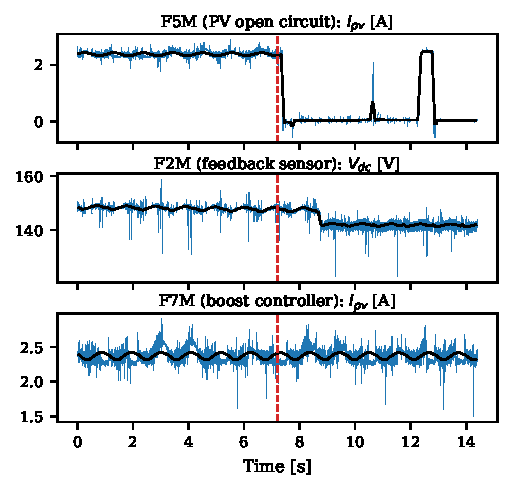
\includegraphics[width=\columnwidth]{figures/signals.pdf}
\caption{Raw signals (blue) and 0.1\,s moving average (black) for three recordings. The dashed red line marks the nominal fault injection at the mid-point of the recording.}
\label{fig:signals}
\end{figure}

\subsection{Windowing and Labels}
Each recording is divided into non-overlapping windows of $W$ samples. The first 0.3\,s are discarded because the magnitude and frequency estimators are initializing. We consider two labeling schemes:
\begin{itemize}
\item \textbf{File labels:} every window of recording F$xy$ receives label $x$, as in~\cite{wali2021explainable}.
\item \textbf{Onset-aware labels:} windows that end before the mid-point $t_o$ receive label 0 (normal), windows that start after $t_o$ receive label $x$, and the few windows straddling $t_o$ are dropped.
\end{itemize}
Only onset-aware labels describe the physical state of the system. With $W=1000$ (0.1\,s, five fundamental cycles) the dataset contains 2{,}109 windows.

\section{Methodology}
\subsection{Features}
\textbf{Statistical signatures (52 features):} mean, standard deviation, minimum and maximum of each of the 13 signals, following~\cite{wali2021explainable}.

\textbf{Physics-informed features (19 features):} PV power $P_{pv}=\overline{I_{pv}V_{pv}}$; AC active power $P_{ac}=\overline{\sum_k v_k i_k}$; conversion ratio $P_{ac}/P_{pv}$; mean $V_{pv}$, $I_{pv}$, $V_{dc}$; ripple (standard deviation) of $V_{dc}$ and $I_{pv}$; mean phase RMS current and voltage; current and voltage unbalance $(\max_k X_k-\min_k X_k)/\bar{X}$ over phase RMS values; zero-sequence current $|\overline{i_a+i_b+i_c}|$; largest per-phase DC offset of the current; current and voltage total harmonic distortion (harmonics 2--13 from the FFT of each window); mean $I_{abc}$, $V_{abc}$; and mean frequency deviation $|V_f-50|$.

\subsection{Baseline Referencing}
Absolute features depend on the operating point: the PV voltage differs by more than 10\,V between the MPPT and IPPT recordings even without faults. A deployed monitor, however, can record a short healthy reference after commissioning or after a change of operating mode. Let $\mu_j$ and $\sigma_j$ be the mean and standard deviation of feature $j$ over the windows of the first $T_{ref}=2$\,s after start-up of the same recording. The referenced feature is
\begin{equation}
z_j=\operatorname{clip}\!\left(\frac{f_j-\mu_j}{\max(\sigma_j,\,10^{-3}|\mu_j|,\,10^{-6})},\,-50,\,50\right).
\label{eq:ref}
\end{equation}
The reference windows are used only for $\mu_j,\sigma_j$ and are excluded from all training and test sets in Protocols P3--P5 below.

\subsection{Classifiers}
We compare logistic regression (LR), a depth-8 decision tree (DT), a 200-tree random forest (RF)~\cite{breiman2001rf}, LightGBM with 200 trees of 15 leaves (LGBM)~\cite{ke2017lightgbm}, and a two-layer multilayer perceptron with 64 and 32 units (MLP), all implemented with scikit-learn~\cite{pedregosa2011sklearn}. Class weights are balanced for LR, DT, RF and LGBM; LR and MLP inputs are standardized. Hyperparameters are fixed a priori to avoid tuning on test data.

\subsection{Evaluation Protocols}
\begin{itemize}
\item \textbf{P1 -- prior protocol:} file labels, $W=200$, statistical features, stratified random 70:30 split of windows~\cite{wali2021explainable}.
\item \textbf{P2 -- sanity check:} as P1, but using only windows that end \emph{before} $t_o$. No fault is physically present, so a diagnosis model should perform at chance level (12.5\% for eight balanced classes).
\item \textbf{P3 -- onset-aware, random:} onset-aware labels, random 70:30 split.
\item \textbf{P4 -- onset-aware, blocked:} for every recording, the pre-fault and post-fault segments are each divided into five contiguous blocks; fold $k$ tests block $k$ of every segment, and training windows within 0.2\,s of a test block of the same recording are purged~\cite{roberts2017cv,bergmeir2012cv}.
\item \textbf{P5 -- cross-mode:} train on all eight MPPT recordings and test on all eight IPPT recordings, and vice versa. Every fault type is thus tested on a recording never seen in training. Predictions of both directions are pooled.
\end{itemize}
We report macro-F1 over the eight classes, per-class recall, the detection rate (fraction of fault windows not classified as normal), and the false-alarm rate (FAR, fraction of normal windows classified as a fault).

\subsection{Training-Free Detection}
Because the referenced features of a healthy system are approximately standard-normal, a simple monitoring statistic is the largest absolute deviation over the 19 physics-informed features, $s=\max_j|z_j|$. The threshold is set to the 99th percentile of $s$ over the reference windows of the eight MPPT recordings only, and an alarm is raised after three consecutive windows exceed it. The detector has no trainable parameters other than the threshold, uses no fault data, and is never calibrated on IPPT data.

\section{Results}
\subsection{The Prior Protocol Rewards Experiment Recognition}
Fig.~\ref{fig:protocols} summarizes the effect of the protocol on the RF. Under P1, the RF reproduces the 100\% accuracy reported in~\cite{wali2021explainable} (LGBM 99.9\%, MLP 99.5\%, DT 98.5\%, LR 96.0\%; MPPT-only RF 99.9\%). Under the sanity check P2 the RF still reaches \textbf{100\%} accuracy and LGBM 99.9\%, although no fault had yet occurred in any of the test windows. Even with blocked cross-validation on the pre-fault data, the RF scores 99.98\%. The classifiers identify the recording, and through it the file label, from the operating point; P1 accuracy is therefore not evidence of fault diagnosis.

\begin{figure}[t]
\centering
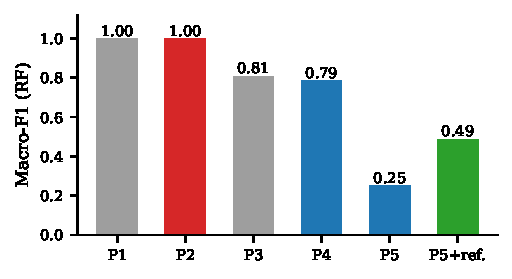
\includegraphics[width=\columnwidth]{figures/protocols.pdf}
\caption{Random-forest macro-F1 under the evaluation protocols of Section~IV-D; ``P5+ref.'' adds baseline referencing. P1/P2 use statistical features with $W=200$; P3 uses statistical and physics features combined; P4--P5 use statistical features with $W=1000$. The red bar (P2) is obtained on pre-fault data only, where a true fault classifier should perform at chance level.}
\label{fig:protocols}
\end{figure}

\subsection{Onset-Aware Labels and Blocked Cross-Validation}
With onset-aware labels the classification problem becomes physically meaningful and performance drops: the best macro-F1 is 0.87 (LGBM) under P3 and 0.85 (LGBM, combined features) under P4 (Table~\ref{tab:main}). These scores hide a large false-alarm rate. Under P4 the RF detects 92\% of fault windows but labels 44\% of normal windows as faults; only 56\% of normal windows are recognized. All 370 false alarms occur in the pre-fault segments of fault recordings, and every one of them is assigned to the fault class of its own recording; none of the 236 windows of the two fault-free recordings is misclassified. This is the same experiment-recognition shortcut. LGBM attains a better trade-off (FAR 14--16\%). Blocked cross-validation removes the leakage between neighboring windows but not the confounding between recording and class, because the remaining blocks of the same recording are still in the training set.

\begin{table}[t]
\caption{Macro-F1 for blocked CV (P4) / cross-mode transfer (P5), $W=1000$. ``ref.'' denotes baseline-referenced features (\ref{eq:ref}).}
\label{tab:main}
\centering
\footnotesize
\setlength{\tabcolsep}{2.4pt}
\begin{tabular}{@{}lccccc@{}}
\toprule
Features & LR & DT & RF & LGBM & MLP \\
\midrule
Stats, raw & 0.72/0.25 & 0.75/0.27 & 0.79/0.25 & 0.83/0.26 & 0.59/0.25 \\
Stats, ref. & 0.62/0.32 & 0.62/0.37 & 0.76/0.49 & 0.75/0.44 & 0.42/0.28 \\
Physics, raw & 0.69/0.17 & 0.74/0.26 & 0.80/0.30 & 0.85/0.24 & 0.53/0.19 \\
Physics, ref. & 0.56/0.34 & 0.55/0.30 & 0.80/0.42 & 0.79/0.39 & 0.42/0.26 \\
Both, raw & 0.73/0.32 & 0.76/0.27 & 0.79/0.23 & 0.85/0.26 & 0.53/0.22 \\
Both, ref. & 0.62/0.37 & 0.60/0.42 & 0.79/0.43 & 0.79/0.43 & 0.42/0.28 \\
\bottomrule
\end{tabular}
\end{table}

\subsection{Cross-Mode Generalization}
P5 is the only protocol in which every fault is diagnosed on a recording the model has never seen. With absolute features, macro-F1 falls to 0.17--0.32 for every model and feature set (Table~\ref{tab:main}), only modestly above the 0.125 chance level. Baseline referencing improves every tree ensemble: the RF rises from 0.25 to 0.49 with statistical features, from 0.30 to 0.42 with physics-informed features and from 0.23 to 0.43 with the combined set, and LGBM from 0.26 to 0.44 with statistical features. The best configuration (RF, referenced statistical features) reaches 0.51 for MPPT$\rightarrow$IPPT and 0.45 for IPPT$\rightarrow$MPPT.

Per-class recall (Table~\ref{tab:perclass}, Fig.~\ref{fig:cm}) shows which faults transfer. The PV open circuit F5 is recognized in 99\% of windows and the feedback-sensor fault F2 in 78\% (0\% without referencing). The inverter fault F1 does not transfer (2\%): in the MPPT recording the mean $V_{pv}$ collapses from 88\,V to 22\,V after the fault and the system shuts down, whereas in the IPPT recording the fault mainly increases the $V_{dc}$ ripple, so the two recordings show different signatures. The inverter fault is instead predicted as F5 (40\%), normal (29\%) or F2 (26\%). The low-magnitude faults F4, F6 and F7 reach only 32--40\% recall; 39--63\% of their windows are classified as normal, and F7 is confused with the related controller fault F6 in 17\% of windows.

\begin{table}[t]
\caption{Per-class recall of the RF. P1: prior protocol; P4: blocked CV (raw stats.); P5: cross-mode with raw and referenced statistical features.}
\label{tab:perclass}
\centering
\footnotesize
\setlength{\tabcolsep}{3pt}
\begin{tabular}{@{}llcccc@{}}
\toprule
 & Class & P1 & P4 & P5 raw & P5 ref. \\
\midrule
N & Normal & 1.00 & 0.56 & 0.86 & 0.82 \\
F1 & Inverter (IGBT) & 1.00 & 0.82 & 0.00 & 0.02 \\
F2 & Feedback sensor & 1.00 & 0.80 & 0.00 & 0.78 \\
F3 & Grid sag & 1.00 & 0.99 & 0.09 & 0.21 \\
F4 & Partial shading & 1.00 & 0.99 & 0.38 & 0.32 \\
F5 & PV open circuit & 1.00 & 0.96 & 0.96 & 0.99 \\
F6 & MPPT/IPPT ctrl. & 1.00 & 0.96 & 0.00 & 0.40 \\
F7 & Boost ctrl. & 1.00 & 0.94 & 0.00 & 0.38 \\
\bottomrule
\end{tabular}
\end{table}

\begin{figure}[t]
\centering
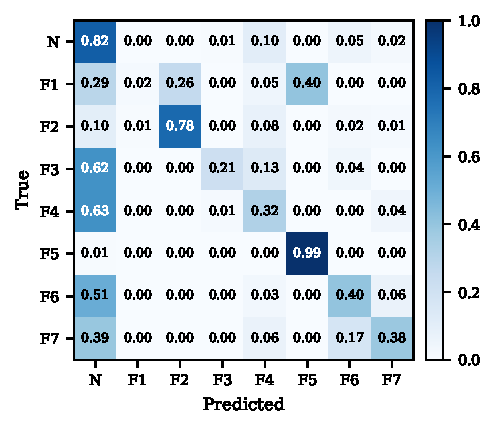
\includegraphics[width=0.9\columnwidth]{figures/confusion_crossmode.pdf}
\caption{Row-normalized confusion matrix of the RF with referenced statistical features under cross-mode transfer (P5, both directions pooled). N: normal.}
\label{fig:cm}
\end{figure}

\subsection{Training-Free Detection}
Table~\ref{tab:detect} and Fig.~\ref{fig:detect} report the training-free detector. Calibrated on MPPT reference windows only, its threshold is $s^\ast=3.65$. On all normal windows outside the reference period, in both modes, the window-level FAR is \textbf{0.7\%}, and no false alarm occurs in the pre-fault segment of any fault recording. The detector flags 97--99\% of post-fault windows for F5, 77--79\% for F2, 67--77\% for F1 and 35--46\% for F7, in both operating modes, although it has never seen a fault or an IPPT recording. Detection delays are measured from the nominal mid-point and are therefore upper bounds; for F2 the visible change itself occurs about 1.5\,s after the mid-point (Fig.~\ref{fig:signals}). The partial-shading fault F4, the controller fault F6 and the grid sags in F3M are not detected at this FAR. Lowering the calibration quantile to 95\% raises F7 detection to 65--80\% and F6 to 14--17\% at a FAR of 4.7\%.

\begin{table}[t]
\caption{Training-free detector (99th-percentile threshold, $K=3$): fraction of post-fault windows flagged and delay of the first alarm after the nominal fault injection, in seconds.}
\label{tab:detect}
\centering
\footnotesize
\setlength{\tabcolsep}{3pt}
\begin{tabular}{@{}llcccc@{}}
\toprule
 & & \multicolumn{2}{c}{IPPT (L)} & \multicolumn{2}{c}{MPPT (M)} \\
\cmidrule(lr){3-4}\cmidrule(lr){5-6}
 & Fault & Rate & Delay & Rate & Delay \\
\midrule
F1 & Inverter (IGBT) & 0.67 & 1.9 & 0.77 & 1.7 \\
F2 & Feedback sensor & 0.77 & 1.8 & 0.79 & 1.7 \\
F3 & Grid sag & 0.24 & 4.0 & 0.00 & -- \\
F4 & Partial shading & 0.00 & -- & 0.00 & -- \\
F5 & PV open circuit & 0.99 & 0.2 & 0.97 & 0.4 \\
F6 & MPPT/IPPT ctrl. & 0.00 & -- & 0.03 & 3.7 \\
F7 & Boost ctrl. & 0.35 & 2.5 & 0.46 & 2.2 \\
\bottomrule
\end{tabular}
\end{table}

\begin{figure}[t]
\centering
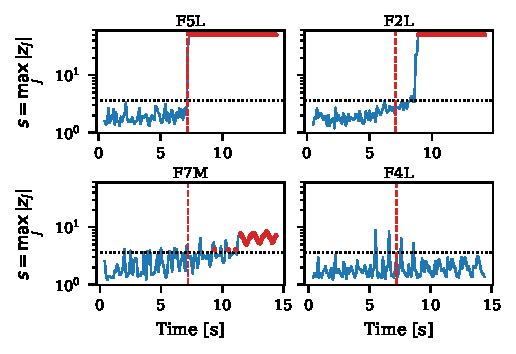
\includegraphics[width=\columnwidth]{figures/detection.pdf}
\caption{Monitoring statistic $s$ (blue), threshold (dotted), nominal fault injection (dashed red) and raised alarms (red dots) for four recordings.}
\label{fig:detect}
\end{figure}

\subsection{Explainability}
Fig.~\ref{fig:shap} shows the mean absolute SHAP values~\cite{lundberg2017shap} of an LGBM trained on referenced physics-informed features. The attributions agree with the physics of each fault. The DC-link voltage deviation is the most informative feature overall, because every fault that disturbs the power balance between the PV array, the boost converter and the inverter moves $V_{dc}$. The feedback-sensor fault F2 is identified mainly through the zero-sequence current $|\overline{i_a+i_b+i_c}|$: a mis-scaled phase sensor makes the three measured currents no longer sum to zero, although the physical currents do. The open circuit F5 is identified through the PV current, partial shading F4 through the PV voltage (a shifted maximum power point), the inverter fault F1 through current unbalance and RMS current, and the MPPT-controller fault F6 through current THD and unbalance. Such explanations allow an operator to check an alarm against the physics of the converter chain before dispatching maintenance.

\begin{figure}[t]
\centering
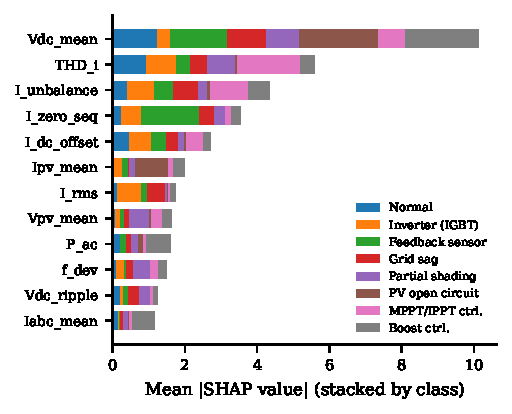
\includegraphics[width=\columnwidth]{figures/shap.pdf}
\caption{Mean absolute SHAP values of the twelve most important referenced physics-informed features, stacked by class (LGBM, all windows).}
\label{fig:shap}
\end{figure}

\subsection{Window Length and Computational Footprint}
Shorter windows help under cross-mode transfer: with referenced physics features and LGBM, macro-F1 decreases from 0.44 at 20\,ms to 0.38 at 500\,ms, while blocked-CV macro-F1 peaks at 0.82 for 50\,ms (Fig.~\ref{fig:window}). Table~\ref{tab:footprint} lists the serialized model size and single-window inference latency on a laptop CPU without a GPU. Extracting the 19 physics-informed features takes 1.2\,ms per 100\,ms window, i.e., about 1.2\% of real time. The depth-8 decision tree requires 7.8\,kB and 0.1\,ms per window, and logistic regression 2.8\,kB, both suitable for a microcontroller in an inverter. The RF (11.6\,MB, 40\,ms including thread-dispatch overhead) and LGBM (2.8\,MB, 1.0\,ms) are considerably heavier while offering the best cross-mode accuracy. The training-free detector stores only the 38 reference statistics $\mu_j,\sigma_j$ and one threshold.

\begin{figure}[t]
\centering
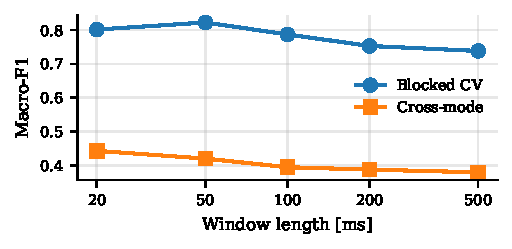
\includegraphics[width=\columnwidth]{figures/window.pdf}
\caption{Effect of the window length on macro-F1 (LGBM, referenced physics-informed features).}
\label{fig:window}
\end{figure}

\begin{table}[t]
\caption{Model footprint (19 referenced physics features, $W=1000$)}
\label{tab:footprint}
\centering
\footnotesize
\begin{tabular}{@{}lcc@{}}
\toprule
Model & Size [kB] & Latency [ms/window] \\
\midrule
LR & 2.8 & 0.299 \\
DT & 7.8 & 0.107 \\
RF & 11643.9 & 39.664 \\
LGBM & 2757.0 & 1.040 \\
MLP & 93.5 & 0.324 \\
\bottomrule
\end{tabular}
\end{table}

\section{Discussion}
\textbf{Implications for benchmarking.} The accuracy obtained under a protocol is an upper bound on what a model has learned about faults only if the protocol excludes shortcuts. On GPVS-Faults, the sanity check P2 is simple to run and shows directly that file-level labels and random splits measure experiment recognition. We recommend that future work on this dataset (i) use onset-aware labels, (ii) report the false-alarm rate alongside accuracy, and (iii) report cross-mode results, which are the closest available proxy for deployment on an unseen installation or operating condition.

\textbf{What can be diagnosed.} Under the strict protocol, severe faults that change the energy flow (F5) or the measured quantities directly (F2) generalize across operating modes, especially with baseline referencing. Inverter faults generalize poorly for classification because their signature depends on the operating mode, but they are still detected by the training-free monitor. Partial shading (F4) and the MPPT controller gain fault (F6) produce changes that are small compared with the natural variation of irradiance and temperature during the recordings, consistent with the observation of the dataset authors that low-magnitude faults are masked by MPPT/IPPT action~\cite{bakdi2020gpvs}.

\textbf{Limitations.} The dataset contains one recording per fault and mode, all from a single laboratory system, so the cross-mode results rest on few independent experiments and cannot be given meaningful confidence intervals. The exact injection instants are not published; we used the documented mid-point, which adds label noise around the onset and makes the reported delays upper bounds. Our hyperparameters were not tuned; tuning on P5 would be optimistic because there is no independent validation recording.

\section{Conclusion}
We showed that the near-perfect accuracies reported on the GPVS-Faults benchmark arise from experiment recognition: a random forest attains 100\% accuracy on data recorded before any fault occurred. Under leakage-aware protocols, eight-class macro-F1 drops to 0.85 within recordings and to 0.17--0.32 across operating modes. Baseline referencing of compact features raises the cross-mode macro-F1 to 0.49, and a training-free detector on the same features transfers across modes with a 0.7\% false-alarm rate while detecting open-circuit, sensor and inverter faults. Reliable diagnosis of partial shading and controller faults remains an open problem that, given the evidence presented here, should be evaluated with cross-recording protocols. Future work will validate the protocol on additional PV fault datasets and investigate detectors for low-magnitude faults that adapt to slow irradiance and temperature variations.

\section*{Data and Code Availability}
The GPVS-Faults dataset is available under CC BY 4.0 at \url{https://doi.org/10.17632/n76t439f65.1}. The code that reproduces all experiments, figures and tables is available at \url{https://github.com/shahihussainofficial1/pv-fault-leakage-benchmark}.

\bibliographystyle{IEEEtran}
\bibliography{references}

\end{document}
